\documentclass[14pt]{matmex-diploma}
%\documentclass[14pt]{matmex-diploma-custom}

\begin{document}
\filltitle{ru}{
    chair              = {Кафедра системного программирования},
    title              = {Разработка механизма использования OpenCL-кода в программах на F\#},
    type               = {coursework},
    position           = {студента},
    group              = 371,
    author             = {Кирилл Петрович Смиренко},
    supervisorPosition = {к.ф.-м.н., доц.},
    supervisor         = {Григорьев С.\,В.}
}
\maketitle

\tableofcontents

% У введения нет номера главы
\section*{Введение}
Графические процессоры (GPU) являются общепринятым средством ускорения вычислений. Многоядерная архитектура видеопроцессоров даёт преимущество в высоконагруженных научных вычислениях, задачах компьютерного зрения, биоинформатики и других областей. Данный подход лёг в основу техники вычислений общего назначения на видеопроцессорах (GPGPU)~\cite{CUDA_to_OpenCL, GPGPU_1}.

Существует ряд технологий для программирования видеопроцессоров. Наиболее распространённой является CUDA --- платформа для параллельных вычислений на видеопроцессорах, разработанная компанией Nvidia в 2007 году~\cite{CUDA}. Другим значимым проектом является Open Computing Language (OpenCL) --- открытый стандарт кросс-платформенного, параллельного программирования различных процессоров, в том числе видопроцессоров, присутствующих в персональных компьютерах, серверах, мобильных и встраиваемых устройствах~\cite{OpenCL}.

Упомянутые технологии предоставляют специальные языки программирования: CUDA C/C++, OpenCL C/C++. В то же время более удобным способом разработки для видеопроцессоров является использование более высокоуровневых языков, таких, как C\# и F\#. Эти языки чаще применяются для написания конечных приложений; кроме того, строгая типизация и статический анализ в интегрированных средах разработки повышают удобство прикладного программирования и надёжность разрабатываемого кода. Уже существует и активно используется ряд средств для высокоуровневого программирования видеопроцессоров~\cite{Brahma_FSharp, FSCL, AleaGPU}.

При этом возникает потребность уметь переиспользовать в языках высокого уровня существующий код на специальных языках для видеопроцессоров. Это продиктовано следующими соображениями. Во-первых, переиспользование готового и проверенного кода вместо переписывания --- стандартная инженерная практика. Во-вторых, низкоуровневый код для видеопроцессоров содержит специфические конструкции, например, барьеры и модификаторы памяти, часто используемые для оптимизаций. Пытаться выразить эти конструкции в языка высокого уровня лишь затем, чтобы потом транслировать их обратно в код целевой платформы (CUDA, OpenCL) для запуска на видеопроцессоре, не представляется рациональным решением.

Таким образом, является актуальной задача переиспользования низкоуровневого кода для GPU в высокоуровневом программировании. При этом отдельный интерес представляет возможность вызова низкоуровневых функций типизированным образом, что существенно повысило бы удобство прикладного программирования.

\section{Обзор}

\subsection{Средства программирования видеопроцессоров}
Существует ряд инструментов, предназначенных для программирования видеопроцессоров на языках программной платформы .NET. Наиболее известные из них представлены ниже.
\begin{itemize}
    \item Alea GPU --- коммерческий продукт от компании QuantAlea, предоставляющий средства разработки для платформы CUDA на языках C\# и F\#~\cite{AleaGPU}.
    \item Brahma.FSharp --- проект с открытым исходным кодом, разрабатываемый на кафедре системного программирования математико-механического факультета СПбГУ. Это транслятор цитируемых выражений языка F\# в код платформы OpenCL~\cite{Brahma_FSharp}.
    \item FSCL --- другой компилятор F\#-кода в OpenCL C с открытым исходным кодом~\cite{FSCL}.
\end{itemize}

Также существуют программные проекты, позволяющие из C\#-кода управлять запуском кода на специальных языках для видеопроцессора. К ним относятся:
\begin{itemize}
    \item Alea GPU, предоставляющий возможность вызова ряда готовых низкоуровневых библиотек~\cite{AleaGPU};
    \item CUSP --- C++-библиотека для вычислений с разреженными матрицами и обработки графов~\cite{CUSP};
    \item ManagedCUDA --- проект, содержащий средства нетипизированного вызова скомпилированных CUDA-функций в коде на C\# и C\#-интерфейс для ряда наиболее популярных CUDA-библиотек.~\cite{ManagedCUDA}.
\end{itemize}

Однако все имеющиеся решения либо только транслируют высокоуровневый код на языках платформы .NET в низкоуровневый код платформ CUDA или OpenCL (Brahma.FSharp, FSCL), либо позволяют использовать лишь фиксированный набор низкоуровневых библиотек (Alea GPU, CUSP). ManagedCUDA является наиболее близким решением, однако не предоставляет типизированных функций вызова низкоуровневого кода и не является транслятором .NET-кода в код платформы CUDA, позволяя работать лишь с предварительно скомпилированной кодовой базой.

В результате обзора можно сделать вывод, что ни одно из существующих решений не позволяет программировать видеопроцессоры на языке высокого уровня и при этом вызывать произвольный низкоуровневый код типизированным образом.

\subsection{Провайдеры типов языка F\#}
Существует несколько способов интеграции низкоуровневого кода и среды исполнения .NET. Особый интерес представляют провайдеры типов F\#~\cite{TypeProviders}. Это механизм языка, который генерирует типы данных и встраивает в окружение времени исполнения как обычные типы F\#. Провайдеры типов могут иметь типовые параметры, и, таким образом, имеется возможность во время разработки на F\# пользоваться статической типизацией данных, которые были получены из динамических источников, например, из файла.

Традиционной и наиболее близкой альтернативой использованию провайдеров типов является кодогенерация. Однако по сравнению с ней провайдеры обладают рядом преимуществ:
\begin{itemize}
    \item провайдеры типов обеспечивают тесную интеграцию с пользовательским контекстом: сгенерированные типы сразу находятся в одном пространстве имён с кодом, который их использует;
    \item генерация типов происходит во время компиляции пользовательского кода, что избавляет от опасности рассинхронизации с источником данных.
\end{itemize}

Провайдеры типов не лишены недостатков. В частности, затруднено тестирование проекта, в котором есть провайдеры типов: тесты, как и любой код, использующий провайдеры, не могут быть включены в ту же сборку, что и провайдер, так как блокируют пересборку последнего. Кроме того, отладка провайдеров типов представляет собой достаточно сложную процедуру, отличающуюся от процесса отладки обычного кода~\cite{TypeProvidersTips}. Тем не менее, данные недостатки относятся к процессу разработки программного решения, но не затрудняют его использование.

Таким образом, именно механизм провайдеров типов F\# был выбран для интеграции разобранного OpenCL-кода и платформы .NET.

\section{Постановка задачи}

Целью данной работы является добавление возможности переиспользования OpenCL C-кода в проект Brahma.FSharp. Для её достижения были поставлены следующие задачи:

\begin{itemize}
    \item исследовать возможности механизма провайдеров типов F\#;
    \item реализовать лексический и синтаксический анализатор заголовков OpenCL-функций;
    \item обеспечить возможность типизированного вызова OpenCL-функций в коде на F\#;
    \item провести экспериментальное исследование представленного решения.
\end{itemize}


\section{Механизм подгрузки OpenCL-кода}

\subsection{Архитектура}
На схеме~\ref{architecture} представлена архитектура предлагаемого решения. Подгружаемый OpenCL C-файл подаётся последовательно лексическому, синтаксическому анализатору и провайдеру типов. На выходе генерируется F\#-тип, содержащий подгруженные функции. Эти функции могут быть использованы в клиентском коде --- цитируемом выражении F\#, которое будет подано существующему транслятору Brahma.FSharp, а результат трансляции --- передан драйверу OpenCL для запуска на видеопроцессоре.

Реализуемый в рамках настоящей работы модуль, таким образом, можно разделить на три составляющих: лексический анализатор, синтаксический анализатор, провайдер типов. Далее будет произведён их подробный обзор.

\begin{figure}[h]
\centering
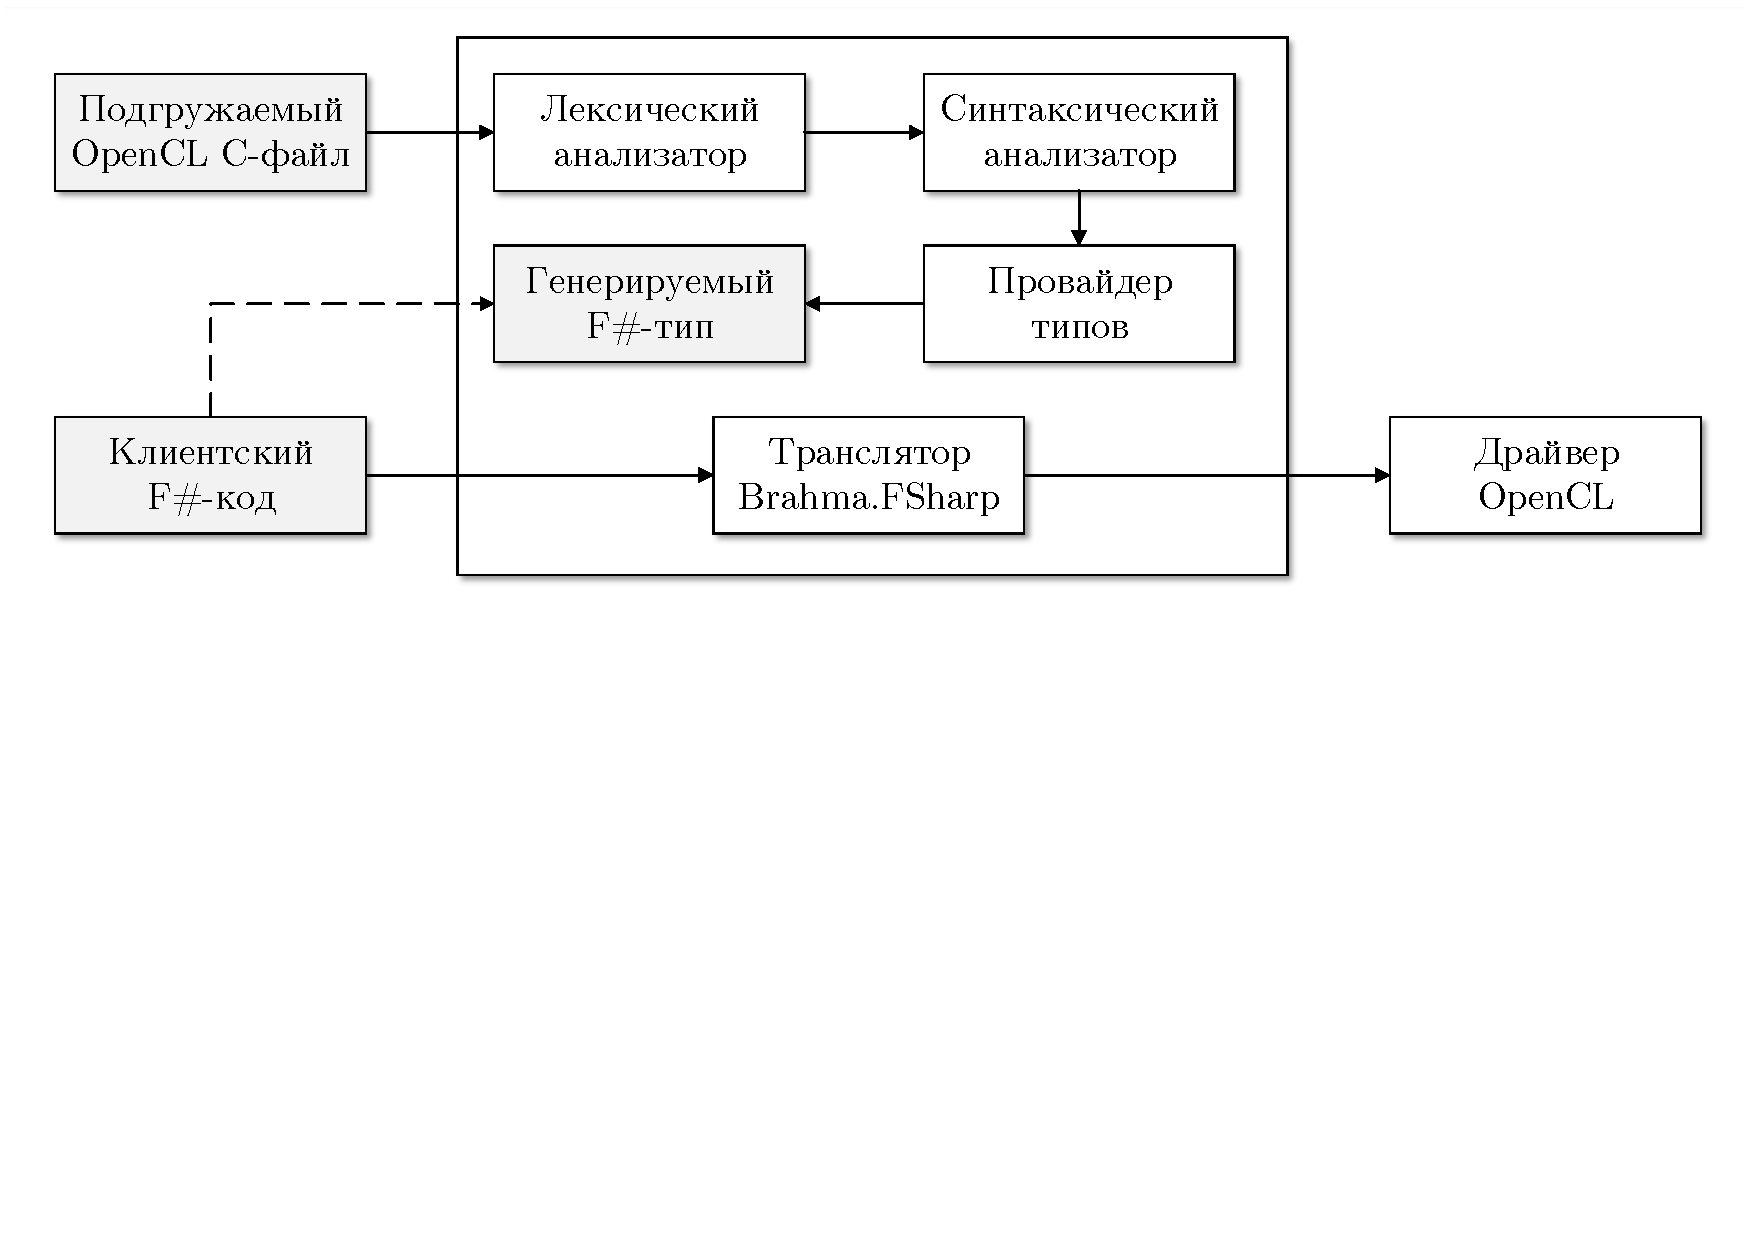
\includegraphics[width=15cm]{courseworkpictures/architecture.pdf}
\caption{Структура предлагаемого решения}
\label{architecture}
\end{figure}

\subsection{Лексический и синтаксический анализатор}
Для того, чтобы извлекать и переиспользовать сигнатуры функций OpenCL C, нужно уметь разбирать исходный код, т.е. проводить лексический и синтаксический анализ. Для реализации лексического анализатора был использован FsLex --- инструмент с открытым исходным кодом, генерирующий исходный код лексических анализаторов на языке F\# по данному описанию языка в специальной нотации~\cite{FsLex}.

При написании синтаксического анализатора была использована библиотека YaccConstructor~\cite{YaccConstructorPaper, YaccConstructorPage}. Она предоставляет язык YARD~\cite{YARD} для описания синтаксических анализаторов. Этот язык имеет ряд преимуществ перед аналогами~\cite{ANTLR, Yacc} применимо к данной задаче: естественная интеграция с F\#, возможность описывать грамматики в расширенной форме Бэкуса-Наура~\cite{EBNF}, поддержка S- и L-атрибутов, а также параметризованных правил вывода.

Синтаксический анализатор описан в виде S-атрибутной грамматики в расширенной форме Бэкуса-Наура. В качестве справочных материалов была использована формальная грамматика C99~\cite{C99} и спецификация языка OpenCL C~\cite{OpenCL_C}. Исходный код обоих анализаторов на F\# генерируется упомянутыми инструментами при сборке проекта.

Представленная грамматика является упрощённой и не описывает весь язык OpenCL C: тот факт, что в данной задаче необходимо распознавать лишь заголовки функций, позволил при разборе игнорировать тела функций.

\subsection{Провайдер типов для OpenCL-функций}
В рамках работы был реализован провайдер типов для разобранных OpenCL-функций. Провайдер генерирует F\#-тип, содержащий функции, которые типизированы так же, как исходные функции на OpenCL C. Провайдер параметризован путём к файлу, содержащему подгружаемый код на OpenCL C; файл может содержать неограниченное количество функций, однострочные комментарии и макросы препроцессора C. Вначале файл с исходным кодом на OpenCL C подвергается лексическому и синтаксическому анализу. Далее производится обход синтаксического дерева, полученного на этапе синтаксического анализа: из дерева извлекаются структурированные сигнатуры функций, по которым провайдер генерирует статические методы предоставляемого метода.

В C-подобных языках, включая OpenCL C, массивы чаще всего передаются по указателям. Поэтому для параметров функций, которые являются указателями, провайдер поддерживает два варианта отображения их в F\#: как ссылочный тип и как массив. Это задаётся другим параметром провайдера. Пример подгрузки с помощью провайдера функции умножения матрицы на вектор представлен на изображении~\ref{tp_call_example}.

\begin{figure}[h]
\centering

\includegraphics[width=15cm]{courseworkpictures/tp-call.png}
\caption{Пример использования провайдера типов}
\label{tp_call_example}
\end{figure}

Также была проведена точечная доработка транслятора\n Brahma.FSharp. Транслятор одновременно с клиентским F\#-кодом получает имя подгружаемого OpenCL C-файла, читает его содержимое и в текстовом виде передаёт драйверу OpenCL вместе с результатом трансляции F\#-кода. Это обеспечивает необходимую функциональность.

\section{Эксперименты}
Помимо модульного тестирования представленного механизма, были произведены экспериментальные исследования работы механизма с высокопроизводительным кодом для видеопроцессора. Это отвечает изначальной мотивации данной работы. В целях эксперимента из стороннего проекта с открытым исходным кодом~\cite{MyGEMM} был взят алгоритм перемножения вещественных матриц на видеопроцессоре, оптимизированный с использованием специфических конструкций OpenCL: барьеров и локальных групп.

Для сравнения производительности были также взяты неоптимизированные реализации наивного алгоритма перемножения матриц на F\# и OpenCL C. Оптимизации, аналогичные таковым в первой рассматриваемой реализации, не представляются возможными в F\# ввиду отсутствия в языке специфических низкоуровневых конструкций. Наивная реализация на OpenCL C участвует в эксперименте с целью сравнения скорости работы OpenCL-кода и аналогичного кода, транслированного из F\#.

Запуск производился средствами Brahma.FSharp на видеокарте\n NVIDIA GeForce GT 755M с тактовой частотой графического процессора 980 МГц и памятью 2048 МБ. Результаты экспериментов представлены на рисунке~\ref{experiments}.

\begin{figure}[h]
\centering
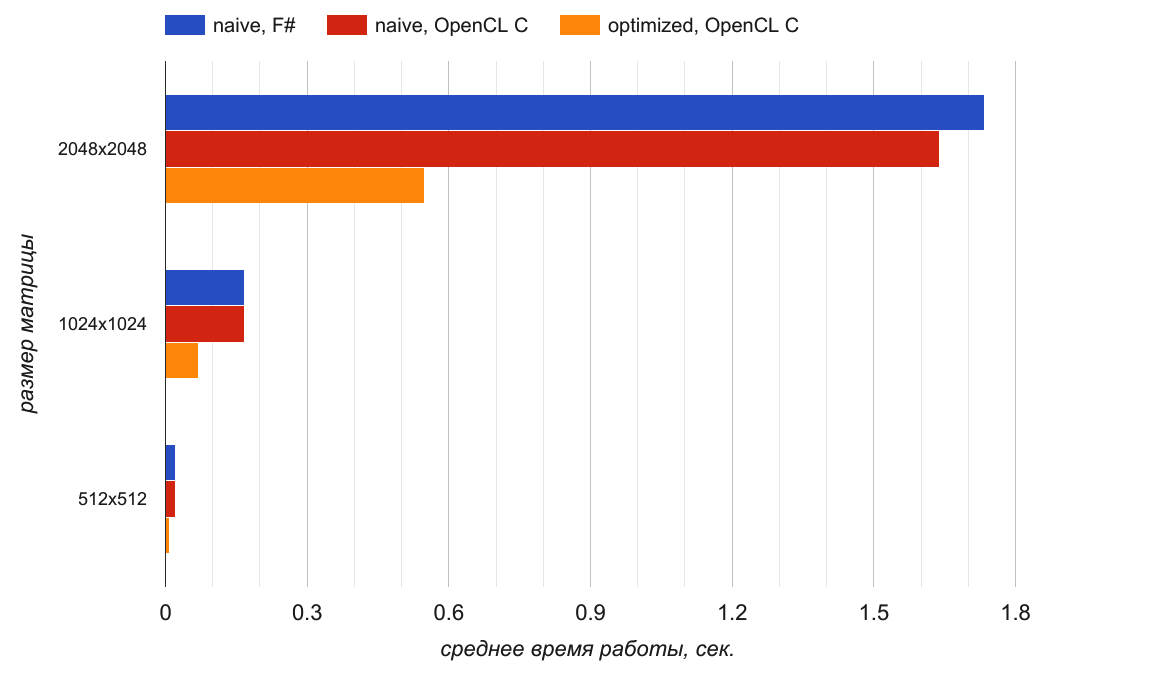
\includegraphics[width=15cm]{courseworkpictures/chart.png}
\caption{Результаты экспериментов}
\label{experiments}
\end{figure}

Как видно на диаграмме, наивные реализации на F\# и OpenCL C почти не отличаются по производительности, в то время как оптимизированная реализация показывает почти трёхкратный прирост производительности на больших матрицах. Это подтверждает целесообразность переиспользования OpenCL-кода, оптимизированного с помощью низкоуровневых конструкций, в высокоуровневом программировании видеопроцессоров.

% У заключения нет номера главы
\section*{Заключение}
В ходе работы получены следующие результаты:
\begin{itemize}
    \item исследован механизм провайдеров типов F\#;
    \item реализован лексический и синтаксический анализатор заголовкой OpenCL-функций;
    \item реализован механизм типизированного вызова OpenCL-функций в коде на F\# на основе провайдера типов;
    \item проведено экспериментальные исследование работы реализованного модуля.
\end{itemize}

Код реализованного модуля, включающего лексический, синтаксический анализатор и провайдер типов, находится на сайте \url{https://github.com/YaccConstructor/Brahma.FSharp}. В указанном репозитории автор принимал участие под учётной записью ksmirenko.

В дальнейшем планируется исследовать возможность применения реализованного механизма при решении задач синтаксического анализа графов с использованием современного алгоритма перемножения разреженных матриц~\cite{SparseMatrixMultiply}. Соответствующий проект разрабатывается на кафедре системного программирования математико-механического факультета СПбГУ.

\setmonofont[Mapping=tex-text]{CMU Typewriter Text}
\bibliographystyle{ugost2008ls}
\bibliography{diploma.bib}
\end{document}
